\documentclass[multi={page}]{standalone}
\usepackage{tikz}
\usetikzlibrary{arrows,positioning}
\tikzset{shorten >=1pt, >=stealth', semithick}
\begin{document}

\begin{page}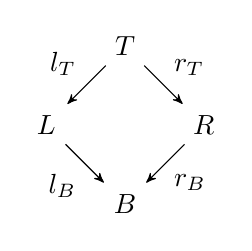
\begin{tikzpicture}

\node (T) at (0,1) {$T$};
\node (L) at (-1,0) {$L$};
\node (R) at (1,0) {$R$};
\node (B) at (0,-1) {$B$};

\draw[->] (T) -- node[above left]{$l_T$} (L);
\draw[->] (T) -- node[above right]{$r_T$} (R);
\draw[->] (L) -- node[below left]{$l_B$} (B);
\draw[->] (R) -- node[below right]{$r_B$} (B);

\end{tikzpicture}\end{page}

\end{document}
